\documentclass[pdf]{beamer}

%\usepackage{lmodern}
\usepackage[font=scriptsize,skip=0pt,justification=justified,singlelinecheck=false]{caption}
%\usepackage{enumitem}
\usepackage{natbib}
\usepackage{bm}
\usepackage{mathtools}
\usepackage[makeroom]{cancel}
\usepackage{minted}

% Using underline
\usepackage{soul}

\usepackage{algorithm}
\usepackage{algpseudocode}
\usepackage{hyperref}
%\usepackage[ruled,vlined]{algorithm2e}
%\usepackage{clrscode3e}


%\usepackage{adjustbox}

%remove the icon
\setbeamertemplate{bibliography item}{}

%remove line breaks
\setbeamertemplate{bibliography entry title}{}
\setbeamertemplate{bibliography entry location}{}
\setbeamertemplate{bibliography entry note}{}
% Use number for caption
\setbeamertemplate{caption}[numbered]{}

\newtheorem{mydef}[theorem]{\Large \underline{\textbf{Definisi}}}

\makeatletter
\def\th@mystyle{%
    \normalfont % body font
    \setbeamercolor{block title example}{bg=blue,fg=white}
    \setbeamercolor{block body example}{bg=blue!20,fg=black}
    \def\inserttheoremblockenv{exampleblock}
  }
\makeatother
\theoremstyle{mystyle}
\newtheorem*{remark}{\textbf{Definition}}


% This file is a solution template for:

% - Talk at a conference/colloquium.
% - Talk length is about 20min.
% - Style is ornate.

% Copyright 2004 by Till Tantau <tantau@users.sourceforge.net>.
%
% In principle, this file can be redistributed and/or modified under
% the terms of the GNU Public License, version 2.
%
% However, this file is supposed to be a template to be modified
% for your own needs. For this reason, if you use this file as a
% template and not specifically distribute it as part of a another
% package/program, I grant the extra permission to freely copy and
% modify this file as you see fit and even to delete this copyright
% notice.  


\mode<presentation>
{
%  \usetheme{AnnArbor} % 
%	\usetheme{Frankfurt}
   \usetheme{Madrid}
  % or ...

%  \setbeamercovered{transparent}
  % or whatever (possibly just delete it)
}


\usepackage[english]{babel}
% or whatever

\usepackage[latin1]{inputenc}
% or whatever

\usepackage{times}
\usepackage[T1]{fontenc}
\usepackage{wasysym}

\usepackage{graphicx} % Necessary to use \scalebox

% Define absolute and norm
\DeclarePairedDelimiter\abs{\lvert}{\rvert}%
\DeclarePairedDelimiter\norm{\lVert}{\rVert}%

% ==============================
%       Redefine emphasize
% ==============================
\let\emph\relax % there's no \RedeclareTextFontCommand
\DeclareTextFontCommand{\emph}{\bfseries\em}


% Swap the definition of \abs* and \norm*, so that \abs
% and \norm resizes the size of the brackets, and the 
% starred version does not.
\makeatletter
\let\oldabs\abs
\def\abs{\@ifstar{\oldabs}{\oldabs*}}
%
\let\oldnorm\norm
\def\norm{\@ifstar{\oldnorm}{\oldnorm*}}
\makeatother

\usepackage{color}
\definecolor{myblue}{rgb}{.8,.8,1}
\usepackage{empheq}
% Or whatever. Note that the encoding and the font should match. If T1
% does not look nice, try deleting the line with the fontenc.

\newlength\mytemplen
\newsavebox\mytempbox

\makeatletter
\newcommand\mybluebox{%
    \@ifnextchar[%]
       {\@mybluebox}%
       {\@mybluebox[0pt]}}

\def\@mybluebox[#1]{%
    \@ifnextchar[%]
       {\@@mybluebox[#1]}%
       {\@@mybluebox[#1][0pt]}}

\def\@@mybluebox[#1][#2]#3{
    \sbox\mytempbox{#3}%
    \mytemplen\ht\mytempbox
    \advance\mytemplen #1\relax
    \ht\mytempbox\mytemplen
    \mytemplen\dp\mytempbox
    \advance\mytemplen #2\relax
    \dp\mytempbox\mytemplen
    \colorbox{myblue}{\hspace{1em}\usebox{\mytempbox}\hspace{1em}}}

\makeatother

\title[Bertahan dalam Pandemi COVID-19] % (optional, use only with long paper titles)
{\textbf{Bertahan dalam Pandemi COVID-19}}

\subtitle
{Kekuatan Doa Menghadapi Krisis~\citep{warren2017fortydays} \\ \textit{2 Tawarikh 20:1-30}}

\author[Hendra Bunyamin] % (optional, use only with lots of authors)
{Hendra Bunyamin}
%{F.~Author\inst{1} \and S.~Another\inst{2}} --> original
% - Give the names in the same order as the appear in the paper.
% - Use the \inst{?} command only if the authors have different
%   affiliation.

\institute[ ] % (optional, but mostly needed)
{
%  \inst{1}%
  Fakultas Ekonomi \\
  Universitas Kristen Maranatha
%  \and
%  \inst{2}%
%  Department of Theoretical Philosophy\\
%  University of Elsewhere
}
% - Use the \inst command only if there are several affiliations.
% - Keep it simple, no one is interested in your street address.

%\date[CFP 2003] % (optional, should be abbreviation of conference name)
%{Conference on Fabulous Presentations, 2003}
% - Either use conference name or its abbreviation.
% - Not really informative to the audience, more for people (including
%   yourself) who are reading the slides online

\subject{Pengantar Teknologi Informasi}
% This is only inserted into the PDF information catalog. Can be left
% out. 

% If you have a file called "university-logo-filename.xxx", where xxx
% is a graphic format that can be processed by latex or pdflatex,
% resp., then you can add a logo as follows:

\pgfdeclareimage[height=1.5cm]{university-logo}{logo-mcu}
\logo{\pgfuseimage{university-logo}}


% Delete this, if you do not want the table of contents to pop up at
% the beginning of each subsection:
\AtBeginSection[]
{
  \begin{frame}<beamer>{Outline}
    \tableofcontents[currentsection,currentsection]
  \end{frame}
}


% If you wish to uncover everything in a step-wise fashion, uncomment
% the following command: 

%\beamerdefaultoverlayspecification{<+->}

\begin{document}

\begin{frame}
  \titlepage
\end{frame}

\begin{frame}{Outline}
  \tableofcontents
  % You might wish to add the option [pausesections]
\end{frame}


% Structuring a talk is a difficult task and the following structure
% may not be suitable. Here are some rules that apply for this
% solution: 

% - Exactly two or three sections (other than the summary).
% - At *most* three subsections per section.
% - Talk about 30s to 2min per frame. So there should be between about
%   15 and 30 frames, all told.

% - A conference audience is likely to know very little of what you
%   are going to talk about. So *simplify*!
% - In a 20min talk, getting the main ideas across is hard
%   enough. Leave out details, even if it means being less precise than
%   you think necessary.
% - If you omit details that are vital to the proof/implementation,
%   just say so once. Everybody will be happy with that.

%\begin{frame}{Make Titles Informative. Use Uppercase Letters.}{Subtitles are optional.}

\section{Kisah Seorang Raja yang Mengalami Krisis Begitu Besar}
\begin{frame}{Siapakah Dia?}
	\begin{figure}[!ht]
		\centering
		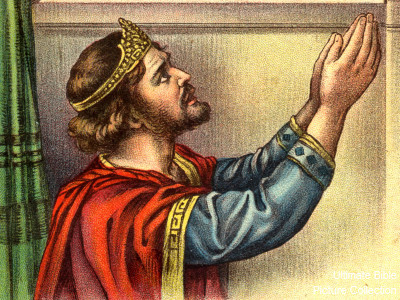
\includegraphics[scale=1.5]{jehoshaphat}
	\end{figure}
	Siapakah Raja di Yehuda ini? \pause \textbf{Raja Yosafat}	
\end{frame}

\begin{frame}{Raja Yosafat menurut \textit{Knowledge Graph} Wikipedia}
	\begin{figure}[!ht]
		\centering
		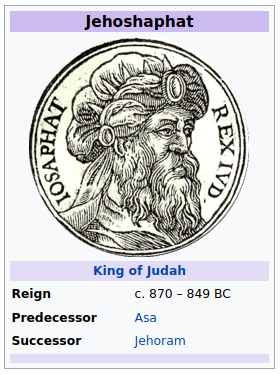
\includegraphics[scale=0.5]{raja-yosafat-wiki}
	\end{figure}
\end{frame}

\begin{frame}{Latar Belakang Raja Yosafat}
	\textbf{2 Tawarikh 17:3-5}: \\
	$^{\bm{3}}$Dan \textit{TUHAN menyertai Yosafat}, karena \textit{ia hidup mengikuti jejak yang dahulu dari Daud, bapa leluhurnya, dan tidak mencari Baal-baal}, \\
	$^{\bm{4}}$melainkan \textit{mencari Allah ayahnya}. Ia hidup menurut perintah-perintah-Nya dan tidak berbuat seperti Israel.\\
	$^{\bm{5}}$Oleh sebab itu TUHAN mengokohkan kerajaan yang ada di bawah kekuasaannya. Seluruh Yehuda memberikan persembahan kepada Yosafat, sehingga ia menjadi \textit{kaya} dan \textit{sangat terhormat}.
\end{frame}

\begin{frame}{Krisis yang Dihadapi Raja Yosafat (1/2)}
	\textbf{2 Tawarikh 20:1-3a}: \\	
	$^{\bm{1}}$Setelah itu bani Moab dan bani Amon datang berperang melawan Yosafat bersama-sama sepasukan orang Meunim. \\
	$^{\bm{2}}$Datanglah orang memberitahukan Yosafat: "Suatu laskar yang besar datang dari seberang Laut Asin, dari Edom, menyerang tuanku. Sekarang mereka di Hazezon-Tamar," yakni \textit{En-Gedi} [dua hari perjalanan jauhnya]. \\
	$^{\bm{3a}}$... Yosafat menjadi takut.
\end{frame}

\begin{frame}{Krisis yang Dihadapi Raja Yosafat (2/2)}
	\begin{figure}[!ht]
		\centering
		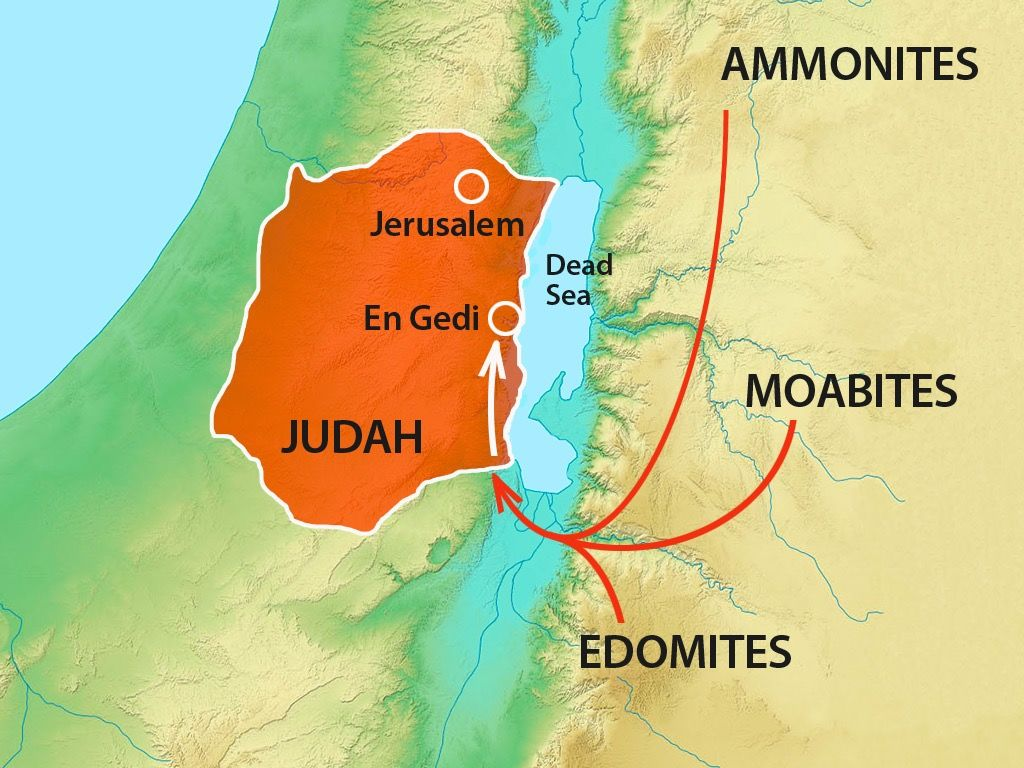
\includegraphics[scale=.27]{jehoshaphat-victory}
\end{figure}		

\end{frame}

\section{Enam Pelajaran dari Sang Raja}
\begin{frame}{1. Berpalinglah kepada $\ldots \ldots$}
	Berpalinglah kepada \textbf{Tuhan untuk mendapat Pertolongan}.
	
	\bigskip
	\textbf{2 Tawarikh 20:3}\\
\textit{	Yosafat menjadi takut, lalu mengambil keputusan untuk mencari TUHAN. Ia menyerukan kepada seluruh Yehuda supaya berpuasa}.
	
	\bigskip	
	
	\begin{itemize}
		\item Daripada membiarkan masalah mengintimidasi kita, jadikan itu motivasi bagi kita untuk \textbf{berdoa}!
		\item Datanglah kepada Tuhan untuk meminta hikmat sebelum kita melakukan hal yang lain.
	\end{itemize}

\end{frame}

\begin{frame}{1. Berpalinglah kepada $\ldots \ldots$}
	Berpalinglah kepada \textbf{Tuhan untuk mendapat Pertolongan}.
	
	\bigskip
	Ingatlah \textbf{betapa besarnya Tuhan itu!}
	
	\bigskip
	\textbf{2 Tawarikh 20:6}: \\
	 "\textit{Ya TUHAN, Allah nenek moyang kami, bukankah Engkau Allah di dalam sorga? Bukankah Engkau memerintah atas segenap kerajaan bangsa? Kuasa dan keperkasaan ada di dalam tangan-Mu, sehingga tidak ada orang yang dapat bertahan melawan Engkau}."	
	
\end{frame}

\begin{frame}{1. Berpalinglah kepada $\ldots \ldots$}
	Berpalinglah kepada \textbf{Tuhan untuk mendapat Pertolongan}.
	
	\bigskip
	Ingatlah \textbf{apa yang telah Tuhan lakukan!}
	
	\bigskip
	\textbf{2 Tawarikh 20:7}: \\
	 "\textit{Bukankah Engkau Allah kami yang menghalau penduduk tanah ini dari depan umat-Mu Israel?}"	
	
\end{frame}

\begin{frame}{1. Berpalinglah kepada $\ldots \ldots$}
	Berpalinglah kepada \textbf{Tuhan untuk mendapat Pertolongan}.
	
	\bigskip
	Ingatlah \textbf{apa yang Tuhan telah janjikan!}
	
	\bigskip
	\textbf{2 Tawarikh 20:7}: \\
	 "\textit{Bukankah Engkau $\ldots \ldots$ memberikan [tanah ini] kepada keturunan Abraham, sahabat-Mu itu, untuk selama-lamanya?}"	
	
\end{frame}

\begin{frame}{1. Berpalinglah kepada $\ldots \ldots$}
	Berpalinglah kepada \textbf{Tuhan untuk mendapat Pertolongan}.
	
	\bigskip
	Mintalah \textbf{sesuai dengan karakter Tuhan!}
	
	\bigskip
	\textbf{2 Tawarikh 20:10-12}: \\
	 $^{\bm{10}}$"\textit{Ketika orang Israel datang dari tanah Mesir, Engkau melarang mereka memasuki negerinya. Oleh sebab itu mereka menjauhinya dan tidak memusnahkannya.}"	 \\
	 $^{\bm{11}}$"\textit{Lihatlah, sebagai pembalasan mereka datang mengusir kami dari tanah milik yang telah Engkau wariskan kepada kami.}" \\
	 $^{\bm{12}}$"\textit{Ya Allah kami, tidakkah Engkau akan menghukum mereka?}"	
\end{frame}

\begin{frame}{2. Akuilah $\ldots \ldots$}
	Akuilah \textbf{keterbatasanmu}.
	
	\bigskip
	\textbf{2 Tawarikh 20:12}: \\
	 $^{\bm{12}}$"\textit{Kami tidak mempunyai kekuatan untuk menghadapi laskar yang besar ini, yang datang menyerang kami. Kami tidak tahu apa yang harus kami lakukan, $\ldots \ldots$}"
	 
	\bigskip

	\textbf{Matius 19:26}: \\
	 $^{\bm{26}}$"\textit{Bagi manusia hal ini tidak mungkin, tetapi bagi Tuhan segala sesuatu mungkin.}"
	 
\end{frame}

\begin{frame}{3. Bersandarlah $\ldots \ldots$}
	Bersandarlah \textbf{kepada kesanggupan Tuhan}.
	
	\bigskip
	\textbf{2 Tawarikh 20:12}: \\
	 $^{\bm{12}}$"\textit{Kami tidak tahu apa yang harus kami lakukan, tetapi mata kami tertuju kepada-Mu}."	 	 
\end{frame}

\begin{frame}{4. Tenanglah $\ldots \ldots$}
	Tenanglah \textbf{dalam iman}.
	
	\bigskip
	\textbf{2 Tawarikh 20:15}: \\
	 $^{\bm{15}}$"\textit{Janganlah kamu takut dan terkejut karena laskar yang besar ini, \textbf{sebab bukan kamu yang akan berperang melainkan Tuhan}}."	 	 \\
	\textbf{2 Tawarikh 20:17}: \\
	 $^{\bm{17}}$"\textit{Dalam peperangan ini tidak usah kamu bertempur. Hai Yehuda dan Yerusalem, tinggallah berdiri di tempatmu, dan \textbf{lihatlah bagaimana TUHAN memberikan kemenangan kepadamu}. Janganlah kamu takut dan terkejut. Majulah besok menghadapi mereka, TUHAN akan menyertai kamu}."	 	 	 \\
	\textbf{2 Tawarikh 20:20}: \\
	 $^{\bm{17}}$"\textit{Percayalah kepada Tuhan, Allahmu, dan kamu akan tetap teguh!}"	 	 	 	 
\end{frame}

\begin{frame}{5. Bersyukurlah kepada Tuhan $\ldots \ldots$ (1/2)}
	Bersyukurlah kepada Tuhan \textbf{terlebih dahulu}.
	
	\bigskip
	\textbf{2 Tawarikh 20:21}: \\
	 $^{\bm{21}}$"\textit{Setelah ia berunding dengan rakyat, ia mengangkat orang-orang yang akan menyanyi nyanyian untuk TUHAN dan memuji TUHAN dalam pakaian kudus yang semarak pada waktu mereka keluar di muka orang-orang bersenjata, sambil berkata: "Nyanyikanlah nyanyian syukur bagi TUHAN, bahwasanya untuk selama-lamanya kasih setia-Nya!}."	 	 
	 
	 \bigskip
	 \begin{itemize}
	 	\item<2-> Bersyukurlah kepada Tuhan atas apa yang akan Ia kerjakan, walaupun kita tak mengerti bagaimana Ia akan melakukannya. 
	 	\item<3-> Jika kita berterima kasih kepada Tuhan setelah ada bukti $\Rightarrow$ \textit{gratitude}. 
	 	\item<4-> Tetapi bila kita berterima kasih sebelum ada bukti $\Rightarrow$ \textit{faith}.
	 \end{itemize}
\end{frame}

\begin{frame}{5. Bersyukurlah kepada Tuhan $\ldots \ldots$ (2/2)}
	Bersyukurlah kepada Tuhan \textbf{terlebih dahulu}.
	
	\bigskip
	\textbf{2 Tawarikh 20:22-23}: \\
	 $^{\bm{22}}$"\textit{Pada waktu paduan suara itu mulai bersorak menyanyi, Tuhan mengadakan kekacauan di tengah-tengah tentara musuh yang sedang menyerang}." \\
	 $^{\bm{23}}$"\textit{Tentara Amon dan Moab menyerang tentara Edom dan menghancurkannya sama sekali. Kemudian mereka balik menyerang satu sama lain dengan sengit}."	 	 	 
\end{frame}

\begin{frame}{6. Harapkan Tuhan $\ldots \ldots$ (1/2)}
	Harapkan Tuhan \textbf{untuk mengubah peperanganmu menjadi berkat}.
	
	\bigskip
	\textbf{2 Tawarikh 20:24-26}: \\
	 $^{\bm{24}}$"\textit{Tidak ada satu musuhpun yang terluput}." \\
	 $^{\bm{25}}$"\textit{Lalu Yosafat dan orang-orangnya turun untuk menjarah barang-barang mereka. Mereka menemukan banyak ternak, harta milik, pakaian dan barang-barang berharga. Yang mereka rampas itu lebih banyak dari pada yang dapat dibawa. Tiga hari lamanya mereka menjarah barang-barang itu, karena begitu banyaknya}." \\
	 $^{\bm{26}}$"\textit{Pada hari keempat mereka berkumpul di Lembah Pujian. Di sanalah mereka memuji TUHAN, dan itulah sebabnya orang menamakan tempat itu Lembah Pujian hingga sekarang}."	 	 	 	 
\end{frame}

\begin{frame}{6. Harapkan Tuhan $\ldots \ldots$ (2/2)}
	Harapkan Tuhan \textbf{untuk mengubah peperanganmu menjadi berkat}.
	
	\bigskip
	Ketika kita membiarkan Tuhan berperang dalam pertempuran kita, hal ini akan menjadi \textbf{kesaksian bagi orang-orang di sekitar kita}.
			
	\bigskip
	\textbf{2 Tawarikh 20:29-30}: \\
	 $^{\bm{29}}$"\textit{Ketakutan yang dari Allah menghinggapi semua kerajaan negeri-negeri lain, ketika mereka mendengar, bahwa TUHAN yang berperang melawan musuh-musuh Israel}." \\
	 $^{\bm{30}}$"\textit{Dan kerajaan Yosafat amanlah, karena Allahnya mengaruniakan keamanan kepadanya di segala penjuru}."
\end{frame}

\begin{frame}[plain]
		\centering
		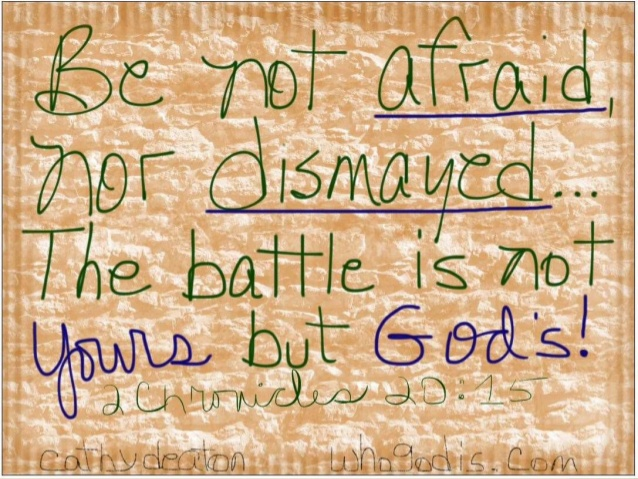
\includegraphics[scale=.5]{the-battle-is-not-yours}
\end{frame}






%\noindent\fbox{%
%    \parbox{\textwidth}{%
%        The quick brown fox jumps right over the lazy dog. 
%    }%
%}











%\begin{frame}{Blocks}
%\begin{block}{Block Title}
%You can also highlight sections of your presentation in a block, with it's own title
%\end{block}
%\begin{theorem}
%There are separate environments for theorems, examples, definitions and proofs.
%\end{theorem}
%\begin{example}
%Here is an example of an example block.
%\end{example}
%\end{frame}


% All of the following is optional and typically not needed. 
\appendix
\section<presentation>*{\appendixname}
\subsection<presentation>*{For Further Reading}

\begin{frame}[allowframebreaks]
  \frametitle<presentation>{Daftar Pustaka}
    {\footnotesize
    \bibliographystyle{apalike}
    \bibliography{references}
    }    
\end{frame}




%\makeatletter % to change template
%    \setbeamertemplate{headline}[default] % not mandatory, but I though it was better to set it blank
%    \def\beamer@entrycode{\vspace*{-\headheight}} % here is the part we are interested in :)
%\makeatother

\begin{frame}[plain]
		\centering
\includegraphics[scale=0.5]{Logo-Maranatha-Untuk-Belakang-02}	
\end{frame}

\end{document}


